\documentclass[conference]{IEEEtran}
\IEEEoverridecommandlockouts
\usepackage[T1]{fontenc}
\usepackage{newtxtext,newtxmath}
\usepackage{amsmath}
\usepackage{graphicx}
\usepackage{booktabs}
\usepackage{array}
\usepackage{multirow}
\usepackage{cite}
\usepackage{url}
\usepackage[hidelinks]{hyperref}
\usepackage{xcolor}
\graphicspath{{figures/}}
% table rows generated by code/analyze.py; the primitive input is expandable,
% so it can be used between \midrule and \bottomrule
\makeatletter\let\inputrows\@@input\makeatother

\newcommand{\repo}{\url{https://github.com/sbsakshi/rl-retail-restocking}}
\DeclareMathOperator*{\argmax}{arg\,max}

\begin{document}

\title{Measuring Reinforcement Learning Against an Exact Optimum: Reward Design, Initialisation and Algorithm Choice for a Retail Shelf-Restocking Robot}

\author{
\IEEEauthorblockN{Sakshi Bansal}
\IEEEauthorblockA{School of Computer Science and Engineering\\
Vellore Institute of Technology, Chennai, India\\
Reg. No. 23BPS1012\\
sakshi.bansal2023@vitstudent.ac.in}
\and
\IEEEauthorblockN{Dr. D. Jeya Mala}
\IEEEauthorblockA{School of Computer Science and Engineering\\
Vellore Institute of Technology, Chennai, India\\
jeyamala.d@vit.ac.in}
}

\maketitle

\begin{abstract}
Hand-designed rewards and default settings shape what a reinforcement-learning agent learns, yet realistic problems offer no optimum to compare against. This paper studies a shelf-restocking robot in a store small enough to solve exactly, and uses the exact optimum to measure both the reward and the learners. The state is reduced to 768 Markov states, an exact model is validated against the simulator, and every policy, tabular or neural, is evaluated exactly on ten store layouts. Dynamic programming shows that the project's original reward pays for walking back and forth near a shelf. Its optimal policy travels 6\% further on average (up to 17\%), at a cost of only 0.3\% of the objective, whereas potential-based versions of the same guidance leave the optimal policy unchanged. Among nine learners trained under four rewards with identical budgets, DQN and Double DQN come closest to the optimum (normalised score 0.96), ahead of PPO (0.79) and every tabular method (at most 0.73). Both bonuses in the original reward help DQN, and their potential-based forms recover about half of that gain. For tabular learners the initial Q-value matters more than the reward: since potential-based shaping is equivalent to initialisation, moving the starting value from 0 to $-150$ triples Q-Learning's score, and direct counts reveal the failure modes on either side. Finally, REINFORCE's argmax policy scores less than half of its stochastic policy, so policy-gradient agents must be evaluated as stochastic policies.
\end{abstract}

\begin{IEEEkeywords}
reinforcement learning, reward shaping, dynamic programming, Q-value initialisation, deep Q-network, retail automation, inventory restocking
\end{IEEEkeywords}

\section{Introduction}
\label{sec:intro}

A shelf that runs empty loses sales until somebody refills it. A restocking robot that decides for itself where to go and when to refill can close that gap, but only if it learns a good policy, and a reinforcement-learning agent learns whatever its reward pays for. The reward is usually designed by hand, with extra terms meant to speed learning up: a bonus for restocking, a bonus for heading toward the emptiest shelf. Whether such terms change what the agent ultimately learns, and how close the agent comes to the best possible policy, are questions that most applied studies cannot answer, because their problems are too large to solve exactly.

This project takes the opposite route. The store, a $4\times4$ grid with a depot, two shelves and a robot that carries two units, is deliberately small enough that the optimal policy can be computed exactly by dynamic programming~\cite{bellman1957,howard1960,puterman1994}. That optimum is then used as a measuring instrument for everything else. Every learned policy, whether a Q-table or a neural network, is evaluated exactly against it, with no sampling noise, on ten store layouts of very different difficulty.

The study builds on the project's earlier reviews, which compared ten algorithm configurations on the same task. Re-examining that work against the exact optimum changed several of its conclusions (Section~\ref{sec:discussion}) and widened the question. Besides asking which algorithm scores highest, this report asks what the reward does to the optimum and why each learner stops where it does.

The contributions are as follows.
\begin{itemize}
\item \emph{An exact reference for a restocking MDP.} The robot's state is reduced to a 768-state Markov tuple, and an exact model is validated against the simulator. Any policy can then be evaluated exactly and scored on a common 0--1 scale across layouts (Section~\ref{sec:problem}).
\item \emph{An exact audit of the reward.} The proposal's bonus for approaching the emptiest shelf is not potential-based, and its optimal policy does exploit the resulting loop, walking 6\% further on average and up to 17\%, at a cost of only 0.3\% of the objective. Potential-based versions of the same guidance leave the optimum unchanged in every state. The discount factor, the travel price and a travel-time bound on service are examined in the same way (Section~\ref{sec:planning}).
\item \emph{A controlled comparison of nine learners under four rewards.} All learners receive the same budget, state and evaluation, and the time limit is treated consistently. DQN trained on the proposal reward comes within a few percent of the optimum. Both proposal bonuses help it, and their potential-based forms recover about half of that help (Section~\ref{sec:results}).
\item \emph{An explanation of the tabular learners' shortfall.} Combining the exact values with Wiewiora's equivalence between shaping and initialisation~\cite{wiewiora2003} shows that the starting Q-value, not the reward, limits the tabular learners. Changing only that value triples Q-Learning's score, and the two failure modes on either side of the best value can be observed directly (Section~\ref{sec:why}).
\end{itemize}

All code, results and notebooks are available at \repo.

\section{Related Work}
\label{sec:related}

\subsection{Reinforcement learning for inventory and warehouse robots}
Inventory control is a long-standing test bed for sequential decision making. Gijsbrechts et al.\ showed that a tuned A3C agent can match strong heuristics and approximate dynamic programming on lost-sales, dual-sourcing and multi-echelon problems~\cite{gijsbrechts2022}, and Boute et al.\ survey the design choices such agents require~\cite{boute2022}. Liu et al.\ coordinate the echelons of a supply chain with heterogeneous-agent PPO~\cite{liu2025}. Closer to the store floor, Jullien et al.\ built RetaiL, a grocery restocking environment from real sales data, and trained a distributional DQN to reduce waste~\cite{jullien2023}. On the robotics side, Zhu et al.\ schedule robots in a mobile fulfilment system with deep RL and metaheuristics~\cite{zhu2024}, and Li et al.\ combine PPO with Dijkstra planning for warehouse navigation~\cite{li2024}. These studies decide \emph{how much} to order or \emph{how} to move; the present task couples the two, since the robot's route determines which shelf can be refilled before it runs out. None of them can say how far their policies are from optimal, because their problems are too large to solve exactly. This study deliberately chooses a store small enough to solve, so that every learned policy can be measured against the true optimum.

\subsection{Reward shaping}
Shaping adds reward for progress toward a goal to speed up learning. Randl{\o}v and Alstr{\o}m found that rewarding progress without penalising regress let a bicycle agent profit from riding in circles~\cite{randlov1998}, a simple instance of what Amodei et al.\ call reward hacking~\cite{amodei2016}. Ng, Harada and Russell proved that shaping of the form $\gamma\Phi(s')-\Phi(s)$ preserves the optimal policy, and that this form is also necessary for the guarantee to hold in every MDP~\cite{ng1999}. Wiewiora then showed that, for tabular TD learners, adding such a term is equivalent to initialising $Q(s,a)$ to $\Phi(s)$~\cite{wiewiora2003}. That equivalence turns out to explain most of what shaping does, and does not do, for the tabular learners in Section~\ref{sec:results}.

\subsection{Evaluation practice}
Henderson et al.\ showed that deep RL results often fail to reproduce across random seeds and implementations~\cite{henderson2018}, and Agarwal et al.\ argued for interval estimates over many runs in place of point estimates~\cite{agarwal2021}. Pardo et al.\ showed that treating a time limit as termination corrupts value estimates and recommended bootstrapping at the cut~\cite{pardo2018}. Van Hasselt traced Q-Learning's weakness in stochastic problems to the overestimation introduced by the max operator~\cite{vanhasselt2010}. All four points apply directly to the agents compared here, and Section~\ref{sec:learning} adopts the corresponding practices.

\section{The Restocking Problem}
\label{sec:problem}

\subsection{Store and robot}
The store is a $4\times4$ grid with a depot at $(0,0)$ and two shelves, each holding up to three units. The robot carries at most two units. At every step it chooses one of seven actions: move up, down, left or right, restock the shelf it stands on, reload at the depot, or wait. Restocking moves as many units as fit from the robot onto the shelf; reloading fills the robot, but only at the depot. After the action, each shelf that still has stock independently loses one unit with probability $p=0.12$, so the two shelves together see on average one sale every four steps. A run is cut after $T=200$ steps. The store does not close at that point, so the cut is a time limit and not a terminal state; Section~\ref{sec:learning} returns to why this distinction matters.

Where the two shelves stand is decided by a layout seed. Ten layouts (seeds 0--9) are used throughout, and each acts as one independent replicate of every experiment. They differ a great deal in difficulty (Fig.~\ref{fig:layouts}): when both shelves are close to the depot almost no sale is ever lost, but when both are five or six cells away the robot cannot keep up with demand.

\begin{figure}[t]
\centering
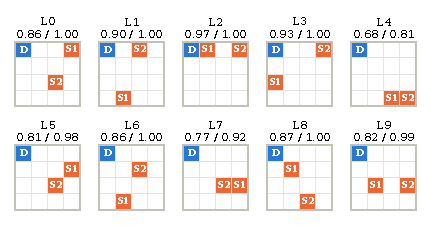
\includegraphics[width=\columnwidth]{layouts}
\caption{The ten store layouts (D: depot; S1, S2: shelves). Each title gives the layout, its optimal service level and the travel-time bound of Section~\ref{sec:bound}.}
\label{fig:layouts}
\end{figure}

\subsection{State}
The Gymnasium observation has eight entries: robot position, units carried, the two stock levels, the number of steps since each shelf was last restocked, and a time-of-day clock. Only the first five affect what happens next. Time since a visit adds nothing once the stock level itself is observed, and demand does not vary with the time of day. The tuple
\begin{equation}
s=(x,\,y,\,c,\,\sigma_1,\,\sigma_2)
\end{equation}
of position, carried units and stock levels is therefore a Markov state, with $4\cdot4\cdot3\cdot4\cdot4=768$ values. Every agent in this study, tabular or neural, observes exactly this tuple. In Review~II the tabular agents also carried a two-valued time-of-day bit, which doubled their table without telling them anything.

\subsection{What the store pays for}
The objective is defined first, before any reward used for training. The store loses sales when a shelf is empty and pays for robot travel, so the objective reward is
\begin{equation}
r_{\text{obj}} = -8\,n_{\text{empty}} - 0.1\,m ,
\label{eq:objective}
\end{equation}
where $n_{\text{empty}}$ counts shelves at zero stock after demand and $m\in\{0,1\}$ records whether the robot moved. A sale is lost only when a customer arrives at an empty shelf, which happens with probability $p$ per step, so the expected number of lost sales is proportional to the number of empty shelf-steps. The weight 0.1 says that 80 moves cost as much as one shelf standing empty for one step; Section~\ref{sec:frontier} examines what that choice implies. Every policy in this paper is scored on~\eqref{eq:objective}, whatever reward it was trained on.

\subsection{The proposal reward}
The project proposal trained agents on a richer signal:
\begin{multline}
r_{\text{prop}} = r_{\text{obj}} - 0.2 - 1\cdot\mathbb{1}[\text{invalid}] + 10\cdot\mathbb{1}[\text{restock}, \sigma>0] \\
+ 5\cdot\mathbb{1}[\text{restock}, \sigma=0] + 2\cdot\mathbb{1}[\text{closer}] ,
\label{eq:proposal}
\end{multline}
with a constant step cost, a penalty for a restock or reload that cannot happen, a bonus for restocking (halved if the shelf was already empty), and a bonus whenever a step reduces the distance to the lowest-stock shelf.

The closer bonus can be gamed. A step toward the target earns $2-0.1-0.2=+1.7$, while a step away costs only $-0.3$, so walking back and forth earns $+1.4$ every two steps where waiting earns $-0.4$. A reward that pays for progress without charging for regress makes loops profitable; Randl{\o}v and Alstr{\o}m observed exactly this when a shaped bicycle controller learned to ride in circles~\cite{randlov1998}. Whether the loop is worth exploiting once stockouts are taken into account is not obvious, and Section~\ref{sec:audit} settles it exactly.

\subsection{Potential-based alternatives}
Ng, Harada and Russell showed that a shaping term of the form
\begin{equation}
F(s,s') = \gamma\,\Phi(s') - \Phi(s)
\label{eq:pbrs}
\end{equation}
leaves the optimal policy unchanged for any bounded potential $\Phi$, because the shaped optimal action values are $Q^\ast(s,a)-\Phi(s)$~\cite{ng1999}. Two potentials are tested. The first keeps the proposal's guidance signal, the same target and the same magnitude, in potential form:
\begin{equation}
\Phi_{d}(s) = -2\, \lVert \text{pos}(s) - \text{shelf}_{\arg\min_i \sigma_i}\rVert_1 .
\end{equation}
The second adds the restock bonus in potential form,
\begin{equation}
\Phi_{ds}(s) = \Phi_d(s) + 5\,(\sigma_1+\sigma_2) ,
\end{equation}
so a two-unit restock pays about $+9.5$ at the moment it happens, close to the proposal's $+10$. The price is that each random sale now also produces a shaping penalty of $-5\gamma$. The four training rewards are referred to as \emph{Proposal}, \emph{Objective}, \emph{PBRS-d} and \emph{PBRS-ds}.

\subsection{Exact model}
Given $(s,a)$, everything except demand is deterministic, and demand has at most $2^2$ outcomes. The model enumerates them into arrays of successor indices, probabilities and reward components, so any of the rewards above is a linear combination of stored arrays. The model was checked against the simulator in three ways, all kept as unit tests: every successor observed in 6{,}000 random transitions exists in the model with the same reward under all four rewards; empirical successor frequencies over 20{,}000 draws agree with the model's probabilities to within four standard errors; and the new simulator, run with the proposal reward, reproduces the Review~II environment to $10^{-15}$ for random action sequences.

\subsection{Exact evaluation and the normalised score}
\label{sec:score}
Because every agent acts on the Markov state, any trained agent, whether a Q-table or a neural network, can be written as a policy $\pi$ over the 768 states. Pushing the start-state distribution forward, $d_{t+1}=d_t P_\pi$, gives the exact expected value of every metric over a 200-step run with no sampling noise. The model is used only to measure; no learner ever sees it. As a cross-check, every final policy is also simulated on 100 demand sequences never used in training; Section~\ref{sec:results} shows that the two measurements agree.

Raw returns from different layouts cannot be averaged, because the layouts differ so much in difficulty. Each policy is therefore placed between a uniform-random policy and the best achievable behaviour:
\begin{equation}
\text{score}(\pi) = \frac{J(\pi) - J(\pi_{\text{rand}})}{J^\ast_T - J(\pi_{\text{rand}})} ,
\label{eq:score}
\end{equation}
where $J$ is the expected 200-step sum of~\eqref{eq:objective} from reset and $J^\ast_T$ is its maximum, obtained by backward induction over the 200 steps. A score of 1 is the best any policy can do in expectation.

\section{What the Exact Optimum Shows}
\label{sec:planning}

\subsection{Value and policy iteration}
Value iteration (VI) on the objective with $\gamma=0.95$ converges to a change below $10^{-10}$ in 441--487 sweeps, about 0.05\,s per layout. Policy iteration (PI), with exact policy evaluation by a linear solve, stops after 13--18 improvement steps. The two value functions agree to $2\times10^{-9}$. Their greedy actions coincide in only 88--96\% of states, however, which matches the unexplained 88.9\% reported in Review~II. The explanation is ties: between 242 and 331 of the 768 states have two or more actions whose values differ by less than $10^{-6}$, usually two moves of equal length toward the same shelf. Counting any optimal action as agreement, PI's policy is optimal for VI in every state of every layout (Table~\ref{tab:layouts}).

\begin{table}[t]
\centering
\caption{Exact solution of each layout under the objective. $SL^\ast$: optimal service level; bound: travel-time bound (Sec.~\ref{sec:bound}); travel: moves per run under $\pi^\ast$; agree: share of states where VI and PI pick the same action; ties: states with more than one optimal action.}
\label{tab:layouts}
\setlength{\tabcolsep}{3pt}
\footnotesize
\begin{tabular}{@{}clcccccccc@{}}
\toprule
L & shelves & $SL^\ast$ & bound & travel & $SL_{\text{rand}}$ & VI & PI & agree & ties\\
\midrule
\inputrows{tables/dp_layouts.tex}
\bottomrule
\end{tabular}
\end{table}

\subsection{Does the training reward change what is optimal?}
\label{sec:audit}
For each training reward the optimal policy was computed and then scored on the objective (Table~\ref{tab:audit}). Three findings follow.

\emph{The closer bonus does pay for itself in travel.} The proposal reward's optimal policy walks 6.1\% further than the objective's on average and 16.8\% further on layout~2. Removing only the closer bonus brings travel back to within 0.3\% of the objective's optimum on average (between $-3.1$\% and $+4.1$\% on individual layouts), and adding only the closer bonus to the objective reproduces the extra travel. The loop described in Section~\ref{sec:problem} therefore matters in practice: an optimal agent under the proposal reward takes it whenever the shelves can spare the time.

\emph{The damage to the objective is small.} The proposal reward's optimal policy still reaches a normalised score of 0.992, against 0.995 for the objective's own optimal policy. The stockout penalty dominates every other term, so an agent cannot afford to loop when a shelf is about to run out. The restock bonus alone barely changes travel, but it makes the optimal action wrong in about 3\% of states: it rewards a top-up for its own sake rather than for the sale it protects. The constant step cost and the invalid-action penalty change nothing, as rows 2 and 3 of Table~\ref{tab:audit} are identical.

\emph{Potential-based shaping is exactly invariant here.} Under both PBRS-d and PBRS-ds the greedy action of the shaped optimum is optimal for the objective in all 768 states of all ten layouts, and the shaped action values equal $Q^\ast-\Phi$ to machine precision, as the theorem predicts~\cite{ng1999}.

\begin{table}[t]
\centering
\caption{Optimal policy of each training reward, scored on the objective (means over 10 layouts). Extra travel is relative to the objective's optimum, with the range over layouts; the last column is the share of states in which the policy's action is optimal for the objective.}
\label{tab:audit}
\setlength{\tabcolsep}{3pt}
\footnotesize
\begin{tabular}{@{}lccccc@{}}
\toprule
optimal policy of & score & $SL$ & travel & extra travel (\%) & opt.\ (\%)\\
\midrule
\inputrows{tables/dp_rewards.tex}
\bottomrule
\end{tabular}
\end{table}

\subsection{The discount factor}
The quantity of interest is the undiscounted 200-step sum, so $\gamma$ is a modelling choice, not part of the problem. Solving the stationary problem for several discounts and scoring each policy against $J^\ast_T$ gives mean scores of 0.983 ($\gamma=0.8$), 0.993 (0.9), 0.995 (0.95), 0.996 (0.98) and 0.999 (0.99). A discount of 0.95, an effective horizon of about 20 steps or two to three round trips, gives up half a percent of the achievable improvement and is used for every learner. A larger discount would recover most of that half percent but would lengthen the horizon over which the learners must propagate values, which Section~\ref{sec:why} identifies as their main difficulty.

\subsection{Service level against travel}
\label{sec:frontier}
Re-solving with move costs between 0 and 8 traces the exact frontier between availability and travel (Fig.~\ref{fig:frontier}). At the chosen price of 0.1 the optimum sits on the flat part of the frontier. On layout~2, raising the price to 0.5 cuts travel from 120 to 107 moves per run while service falls from 0.969 to 0.968. If robot energy has a real cost to the store, the proposal's weight undervalues it; the frontier lets that decision be taken knowingly.

\subsection{A bound from travel time}
\label{sec:bound}
Each unit sold from shelf $i$ must first be carried there. A reload, trip, restock and return carrying two units takes $2d_i+2$ steps, where $d_i$ is the shelf's distance from the depot, so each delivered unit costs at least $d_i+1$ steps of robot time; splitting a load between shelves is never cheaper per unit. Expected sales from shelf $i$ are at least $pT\,SL_i$ and cannot exceed its initial three units plus what is delivered. Hence
\begin{equation}
\sum_i (d_i+1)\,\max\bigl(0,\; pT\,SL_i-3\bigr) \le T + d_{\max} + 2 ,
\end{equation}
where the slack allows for the robot starting loaded and not returning after its last trip. Maximising the mean $SL_i$ under this constraint is a small linear program. The bound binds only when both shelves are far from the depot (Table~\ref{tab:layouts}). On layout~4, with shelves five and six cells away, no policy can exceed a service level of 0.807 and the optimum reaches 0.683. Elsewhere the bound is 0.98 or more, and what limits the optimum is the randomness of demand, not the robot's capacity.

\section{Learning Agents and Protocol}
\label{sec:learning}

\subsection{Agents}
Nine learners are compared. They are grouped by how they turn experience into an update, because that is the property the results turn on.

\emph{One-step temporal-difference control.} Q-Learning~\cite{watkins1992} moves $Q(s,a)$ toward $r+\gamma\max_{a'}Q(s',a')$ and is off-policy. SARSA~\cite{rummery1994} uses $r+\gamma Q(s',a')$ for the action actually taken next and is on-policy.

\emph{Multi-step and Monte Carlo control.} 4-step Sarsa replaces the one-step target with four observed rewards plus $\gamma^4Q(s_{t+4},a_{t+4})$~\cite{sutton2018}. SARSA($\lambda$) with $\lambda=0.8$ applies every TD error to all recently visited pairs through accumulating eligibility traces, pruned once they fall below $10^{-3}$. Every-visit Monte Carlo control moves $Q$ toward the observed discounted return and never bootstraps inside an episode.

\emph{Function approximation.} DQN~\cite{mnih2015} learns $Q_\theta$ from a replay buffer against a periodically copied target network; Double DQN~\cite{vanhasselt2016} lets the online network choose the next action and the target network evaluate it, to reduce overestimation. REINFORCE with a learned baseline~\cite{williams1992} raises the log-probability of each action in proportion to its return minus a value estimate. PPO~\cite{schulman2017} reuses each batch for several epochs under a clipped probability-ratio objective, with advantages from generalised advantage estimation~\cite{schulman2016}.

\subsection{Shared settings}
Every learner receives the same budget, 600 runs of 200 steps (120{,}000 environment steps), the same discount $\gamma=0.95$, and the same five-number Markov state. Tabular agents use a $768\times7$ table; all networks have two hidden layers of 64 ReLU units and see the state scaled to $[0,1]$. Value-based agents explore $\varepsilon$-greedily, with $\varepsilon$ falling linearly from 1 to 0.05 over the first 450 runs and then held, so every method ends with the same consolidation phase. Table~\ref{tab:hyper} lists the remaining settings. The DQN and PPO settings are the published defaults of each method~\cite{mnih2015,schulman2017}, scaled to this budget, and were not tuned, so that no algorithm benefits from a larger tuning effort than the others. REINFORCE is the one exception. It has no widely used default, and pooling ten runs per update left only 60 gradient steps in the budget, after which its policy was still at chance level. It therefore uses the textbook single update per run, with the policy learning rate chosen from $\{10^{-3}, 3\cdot10^{-3}, 10^{-2}\}$ on three layouts.

\begin{table}[t]
\centering
\caption{Hyperparameters. All learners: 120{,}000 steps, $\gamma=0.95$, same Markov state input.}
\label{tab:hyper}
\footnotesize
\setlength{\tabcolsep}{4pt}
\begin{tabular}{@{}l>{\raggedright\arraybackslash}p{0.6\columnwidth}@{}}
\toprule
Tabular (all five) & $\alpha=0.15$ constant, $Q_0=0$, $\varepsilon$: $1\to0.05$\\
4-step Sarsa / SARSA($\lambda$) & $n=4$ / $\lambda=0.8$, trace cut-off $10^{-3}$\\
DQN, Double DQN & Adam $5\cdot10^{-4}$, batch 64, buffer 50k,\\
& target copied every 500 steps, Huber loss\\
REINFORCE + baseline & Adam $3\cdot10^{-3}$ (policy), $10^{-3}$ (value),\\
& one update per run, entropy 0.01\\
PPO & Adam $3\cdot10^{-4}$, rollout 2048, 10 epochs, batch 64,\\
& clip 0.2, GAE $\lambda=0.95$, entropy 0.01\\
Networks & 2 $\times$ 64 ReLU; rewards scaled by 0.1 in updates\\
\bottomrule
\end{tabular}
\end{table}

\subsection{The time limit is not a terminal state}
Because the store keeps running after step 200, treating the cut as terminal would teach every agent that the last few states of a run are worth nothing, which is false and, since the state does not include the clock, inconsistent with the same states seen earlier in a run. Following Pardo et al.~\cite{pardo2018}, every target that reaches the limit bootstraps from the value of the state the run was cut in: the one-step and trace methods do so naturally, 4-step Sarsa bootstraps its last windows from $Q(s_T,a_T)$, Monte Carlo adds $\gamma^{T-t}Q(s_T,a_T)$ to its returns, REINFORCE adds $\gamma^{T-t}V(s_T)$, PPO's advantage estimate starts from $V(s_T)$, and DQN stores no done flag at all. Review~II's DQN treated the cut as terminal, and its Monte Carlo and $n$-step agents dropped the tail; all three are corrected here.

\subsection{Measurement and statistics}
Each greedy policy is evaluated exactly (Section~\ref{sec:score}) every 20 runs during training and once at the end. For the two policy-gradient methods both the greedy policy and the stochastic policy they actually learned are evaluated, since the two can behave very differently. Each experiment is replicated over the ten layouts, with one training run per layout; intervals are 95\% $t$-intervals over layouts. Comparisons between training rewards are paired by layout, since the same store and the same random seed are used for each reward, and are tested with a paired $t$-test on the per-layout differences. This follows the advice of Henderson et al.~\cite{henderson2018} and Agarwal et al.~\cite{agarwal2021} to report uncertainty across independent runs, not a single best run.

\section{Results}
\label{sec:results}

Every learner was trained under every reward on every layout: nine learners, four rewards and ten layouts in the main grid (360 runs), plus the follow-up runs described below. Across all 730 runs, the simulated check agreed with exact evaluation as expected if both are correct (standardised difference: mean 0.24, standard deviation 1.01, $|z|>2$ in 5.2\% of runs).

\subsection{Overall comparison}
Table~\ref{tab:scores} and Fig.~\ref{fig:reward} give the final normalised scores. Three groups stand out.

\emph{DQN and Double DQN} are the strongest learners under every reward and come close to the optimum when trained on the Proposal reward (0.96 for both). They beat the best tabular method, SARSA($\lambda$), on every reward (paired $p<0.001$), and they learn fastest: half of the achievable improvement is reached after a median of 24{,}000--34{,}000 steps, against 72{,}000--76{,}000 for SARSA($\lambda$) (Fig.~\ref{fig:curves}). Double DQN is never significantly different from DQN ($p\ge0.16$). Its correction for overestimation has little to correct in a problem this small.

\emph{PPO} reaches 0.73--0.79, with much wider intervals than DQN: it solves some layouts almost perfectly and stalls on others. With the same 120{,}000 steps, an on-policy method that discards its data after each update is at a disadvantage against a replay-based one, and the learning curves are still rising when the budget ends.

\emph{The tabular learners} spread from Q-Learning (0.17--0.27) to SARSA($\lambda$) (0.63--0.73), in the order that the amount of credit assignment per update would suggest: multi-step and trace methods above one-step SARSA, and Q-Learning last. Monte Carlo control is the least sensitive to the reward and is never better than 0.43. REINFORCE with a baseline is the weakest learner by its greedy policy (0.04--0.22), but Section~\ref{sec:stochastic} shows that this figure understates what it learned.

\begin{table}[t]
\centering
\caption{Final normalised score by learner and training reward (mean $\pm$ 95\% CI over 10 layouts; 0 = random, 1 = best achievable). Bold: best reward for the learner. $^\ast$: different from Objective, paired $t$-test, $p<0.05$.}
\label{tab:scores}
\setlength{\tabcolsep}{2.5pt}
\footnotesize
\begin{tabular}{@{}lcccc@{}}
\toprule
learner & Proposal & Objective & PBRS-d & PBRS-ds\\
\midrule
\inputrows{tables/scores.tex}
\bottomrule
\end{tabular}
\end{table}

\begin{figure*}[t]
\centering
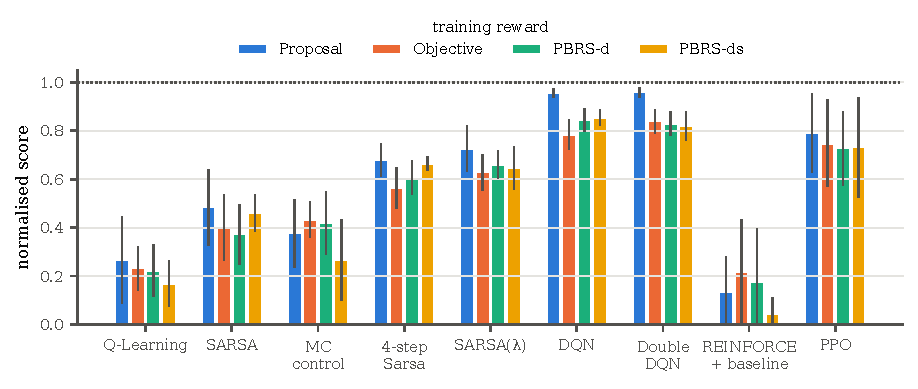
\includegraphics[width=\textwidth]{reward_effect}
\caption{Final normalised score of every learner under each training reward (mean and 95\% CI over 10 layouts). The dotted line is the best achievable behaviour.}
\label{fig:reward}
\end{figure*}

\begin{figure*}[t]
\centering
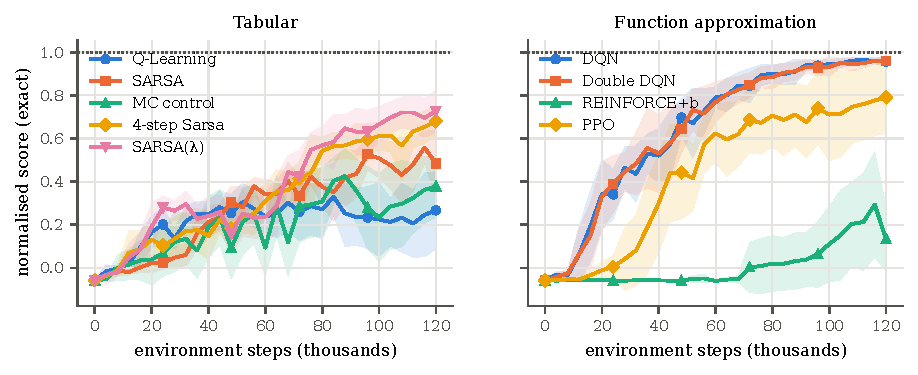
\includegraphics[width=\textwidth]{curves_proposal}
\caption{Learning curves under the Proposal reward: the exact normalised score of the current greedy policy every 20 runs (mean and 95\% CI over 10 layouts).}
\label{fig:curves}
\end{figure*}

\subsection{Operational metrics}
Table~\ref{tab:metrics} translates the scores into the six measures named in the project proposal, each defined so that it can be computed exactly: cumulative objective reward, service level (task completion), travel (energy), mean stockout duration (response time, the number of empty shelf-steps per shelf that ran out), load factor (resource utilisation, units per restock as a share of capacity) and, in Fig.~\ref{fig:curves}, convergence speed. DQN keeps shelves stocked 82\% of the time against 84.5\% for the optimum, and refills an empty shelf after 6.4 steps on average against 6.3. PPO shows how a mean can mislead: it has the largest share of proactive restocks, yet its mean stockout lasts 41 steps, because on the layouts where it stalls an empty shelf stays empty for most of the run. The tabular learners leave shelves empty for 11--67 steps.

\begin{table}[t]
\centering
\caption{Expected metrics per 200-step run for learners trained on the Proposal reward, beside the optimal policy (means over 10 layouts). $J$: objective; SL: service level; travel: moves; stockout: mean stockout duration (steps); proact.: share of restocks made before the shelf ran out; load: units per restock / capacity; opt.: probability of an optimal action on states $\pi^\ast$ visits.}
\label{tab:metrics}
\setlength{\tabcolsep}{2pt}
\footnotesize
\begin{tabular}{@{}lcccccccc@{}}
\toprule
 & score & $J$ & SL & travel & stockout & proact. & load & opt.\\
\midrule
\inputrows{tables/metrics_proposal.tex}
\bottomrule
\end{tabular}
\end{table}

\subsection{Which reward trains best, and why}
\label{sec:which}
Section~\ref{sec:audit} showed that the Proposal reward is slightly wrong at the optimum. Here it is the best training signal for seven of the nine learners, significantly so for 4-step Sarsa, SARSA($\lambda$), DQN and Double DQN (Table~\ref{tab:scores}). To find out which part of it helps, the restock bonus and the closer bonus were each added to the objective on their own (Table~\ref{tab:terms}).

For DQN both terms help, by $+0.12$ and $+0.10$, and the reward containing both reaches 0.96, up from 0.78. Their potential-based counterparts (PBRS-ds and PBRS-d) recover roughly half of each gain while provably leaving the optimal policy unchanged. The price of the larger gain is visible in behaviour: DQN trained on the Proposal reward travels further than the optimal policy on nine of the ten layouts. On layout~2, DQN and PPO both make about 140 moves per run where the optimum makes 120, and they sit to the right of the exact frontier (Fig.~\ref{fig:frontier}). The learners take the same loop that costs an optimal agent 0.3\% in score, and in exchange they reach a far better policy within the budget. At this training budget the Proposal reward is therefore the better choice, and the exact audit says what it costs.

\begin{table}[t]
\centering
\caption{One proposal term at a time (final score, mean of 10 layouts). $^\ast$: paired $p<0.05$ against Objective.}
\label{tab:terms}
\setlength{\tabcolsep}{2.2pt}
\footnotesize
\begin{tabular}{@{}lcccccc@{}}
\toprule
learner & Obj. & +restock & +closer & Proposal & PBRS-d & PBRS-ds\\
\midrule
\inputrows{tables/terms.tex}
\bottomrule
\end{tabular}
\end{table}

\begin{figure*}[t]
\centering
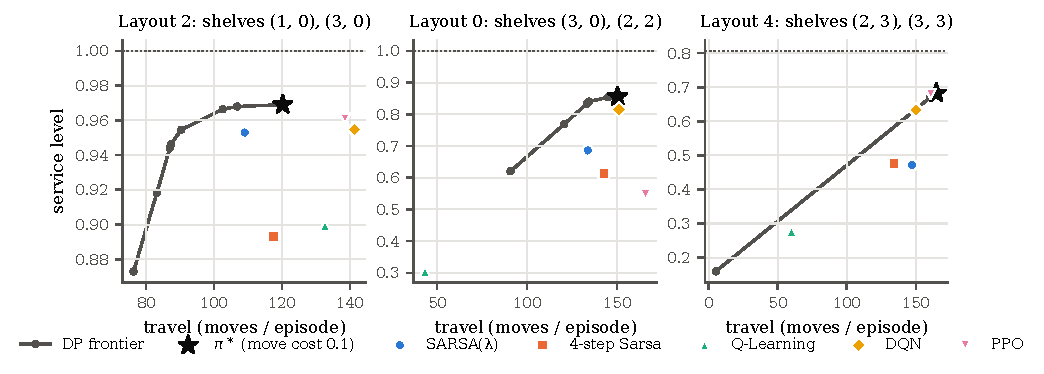
\includegraphics[width=\textwidth]{frontier_proposal}
\caption{Learned policies (Proposal reward) against the exact service--travel frontier of three layouts. The star is the optimum at the objective's travel price, and the dotted line is the travel-time bound. Points to the right of the frontier travel more than necessary for their service level.}
\label{fig:frontier}
\end{figure*}

\subsection{Why the tabular learners fall short}
\label{sec:why}
For the tabular learners, the reward explains less than it seems to. All five start from $Q_0=0$, and since the objective only ever charges, zero is above the optimal value of every state. Fig.~\ref{fig:diag} (left) measures how much of that optimism is left after training, as the gap between the learned values and $V^\ast$ on the states the optimal policy visits. One-step Q-Learning and SARSA still sit about 37--39 above $V^\ast$ after 120{,}000 steps: each update moves a value only a fraction $\alpha$ of the way toward a target that is itself too high. Eligibility traces and multi-step targets pass each correction back through many states at once and remove most of the gap (SARSA($\lambda$): $+7$). Monte Carlo, which never bootstraps, ends below $V^\ast$. Across layouts, the remaining optimism goes with a lower score.

Wiewiora's result~\cite{wiewiora2003} shows why shaping cannot remove this gap. For a tabular learner, adding $\gamma\Phi(s')-\Phi(s)$ to every reward is the same as starting from $Q_0(s,a)=\Phi(s)$. This was confirmed directly: with identical seeds, SARSA on PBRS-d and SARSA on the objective started from $\Phi$ visit the same states and keep tables that differ by exactly $\Phi(s)$ to $3\times10^{-14}$ for all 600 runs. PBRS-d therefore only lowers the starting values by twice the distance to the target shelf, at most 12, against an optimism of about 50, which is why it barely moves the tabular scores. The Proposal reward helps them for a related reason: its bonuses raise the true values, so the zero start is only about 20 above them instead of 55.

The causal test is to keep the objective and change only $Q_0$ (Table~\ref{tab:init}, Fig.~\ref{fig:init}). Starting at $-150$ triples Q-Learning's score (0.23 to 0.69) and lifts every TD learner significantly above its $Q_0=0$ result ($p\le0.001$). It also beats the Proposal reward started at zero, significantly for Q-Learning, SARSA and 4-step Sarsa ($p<0.01$) and narrowly for SARSA($\lambda$) (0.79 against 0.73, $p=0.10$). The effect has an inverted-U shape, with two failure modes that can be observed directly. Counting state--action visits during training on five layouts: with $Q_0=0$, the greedy action is the least-tried action in its state 9--16\% of the time, so the policy is pulled toward the actions it knows least about. With $Q_0=-300$ that never happens, but the greedy action has been tried thousands of times: the policy has locked onto early choices instead of comparing alternatives. The best constant, $-150$, lies close to the mean optimal value of the states an exploring agent visits ($-137$), between the largest ($-19$) and smallest ($-197$) optimal values. This is an observed coincidence, not a derived rule. Even at the best value, $Q_0=-150$, the trained values sit 67--82 \emph{below} $V^\ast$, so the greedy policy depends on how the leftover error is spread across the actions of a state more than on how accurate the values are. Monte Carlo is insensitive to $Q_0$, as expected for a method that never bootstraps.

\begin{figure*}[t]
\centering
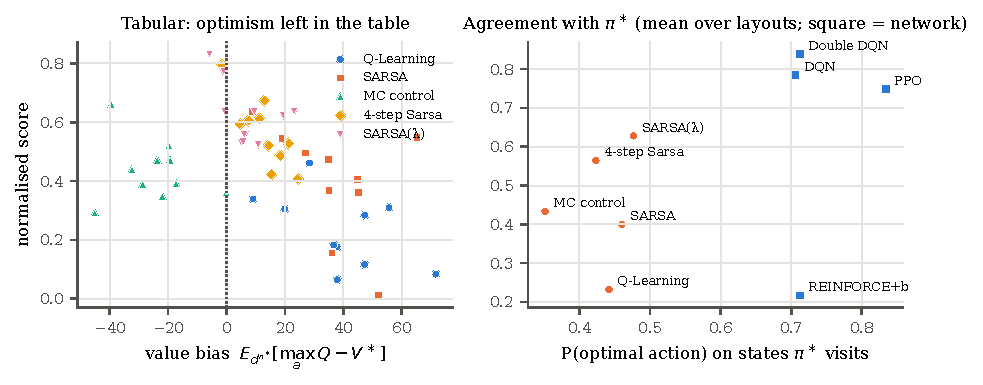
\includegraphics[width=\textwidth]{diagnostics_objective}
\caption{Inside the learned policies (Objective reward). Left: optimism left in each Q-table after training (one point per layout). Right: probability of choosing an optimal action on the states the optimal policy visits, against the score (one point per learner).}
\label{fig:diag}
\end{figure*}

\begin{figure}[t]
\centering
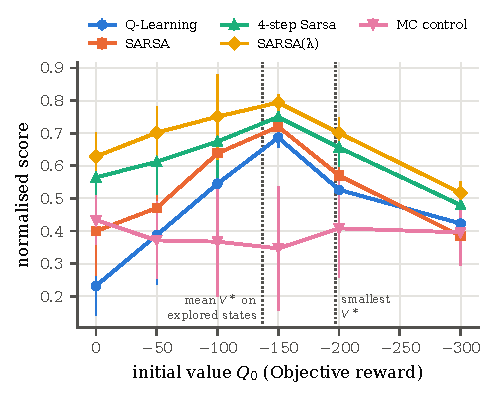
\includegraphics[width=\columnwidth]{init}
\caption{Tabular learners on the Objective reward with different initial values (mean and 95\% CI over 10 layouts). Dotted lines: mean optimal value of states an exploring agent visits, and the smallest optimal value.}
\label{fig:init}
\end{figure}

\begin{table}[t]
\centering
\caption{Final score on the Objective reward for initial values $Q_0$ (mean of 10 layouts; bold: best). For DQN, $Q_0$ is set through the output bias. Last column: Proposal reward with $Q_0=0$, for comparison.}
\label{tab:init}
\setlength{\tabcolsep}{2.4pt}
\footnotesize
\begin{tabular}{@{}lccccccc@{}}
\toprule
learner & 0 & $-50$ & $-100$ & $-150$ & $-200$ & $-300$ & Prop.\\
\midrule
\inputrows{tables/init.tex}
\bottomrule
\end{tabular}
\end{table}

None of this applies to DQN. Setting its output bias so that every initial value is $-150$ changes nothing for DQN (0.79 against 0.78, $p=0.80$) and makes Double DQN slightly worse (0.78 against 0.84, $p=0.02$). A network shares its parameters across states, so a few hundred updates rescale every output at once and no state keeps its initial value for long. For DQN, the gain from the Proposal reward is a genuine effect of its extra terms, as Table~\ref{tab:terms} showed.

\subsection{Greedy or stochastic policy-gradient agents}
\label{sec:stochastic}
REINFORCE and PPO learn a stochastic policy, and both forms were evaluated exactly. For REINFORCE the difference is large: its stochastic policy scores 0.45--0.49, while the argmax of the same policy scores 0.27--0.41 lower under every reward ($p\le0.012$). Reporting the argmax alone would understate what REINFORCE learned by more than half. For PPO the two forms agree on average (mean differences between $-0.04$ and $+0.03$), but on single layouts the gap reaches 0.62. Policy-gradient agents should therefore be evaluated with their stochastic policies.

\section{Discussion}
\label{sec:discussion}

\subsection{Corrections to the earlier reviews}
Measuring every policy against the optimum, on every layout, with identical budgets, changed several conclusions of Review~II. They are listed here so the two reports can be read together.

\emph{The PPO ``overfitting'' case.} Review~II reported a PPO run that reached 81\% completion during training but 18.6\% on held-out demand, and attributed the gap to overfitting a demand sequence. That explanation cannot hold, since every training run already used a fresh demand seed. The training curve was computed from the sampled stochastic policy, whereas the held-out figure came from its argmax, and the argmax of an undertrained stochastic policy can be very different from the policy itself. With both forms evaluated exactly, PPO's greedy and stochastic policies here differ by at most 0.04 in normalised score on average, although by up to 0.62 on a single layout, and REINFORCE's argmax scores 0.27--0.41 below its own stochastic policy (Section~\ref{sec:stochastic}).

\emph{REINFORCE's energy result.} REINFORCE was trained on 60-step runs while every other method used 200, so its travel and return figures were not comparable; its apparent energy efficiency reflected shorter runs and a policy that barely moved. All learners now use identical runs.

\emph{The 88.9\% VI/PI agreement} is fully explained by ties (Section~\ref{sec:planning}); the two methods agree exactly.

\emph{The time limit.} Review~II's DQN treated step 200 as a terminal state, and its Monte Carlo and $n$-step agents ignored what lay beyond it; both bias the values of late states.

\emph{Layouts and seeds.} Each training seed was also a different store, so seed-to-seed variance mixed algorithmic noise with layout difficulty, and the dynamic-programming reference existed for one layout only. Per-layout optima and the normalised score separate the two.

\emph{The tabular state} carried a time-of-day bit that no part of the dynamics reads; it doubled the table without adding information.

\subsection{Limitations}
The store is small by design; that is what makes an exact optimum available. The tabular methods would not scale to a realistic store, and the absolute scores of the deep agents on this small problem say little about their behaviour on a large one. What should carry over is the method: build a version of the problem small enough to solve, and use it to check reward design and learner behaviour before scaling up.

Each layout received one training run per configuration, so the intervals combine layout and seed variation; with ten layouts this is enough to separate the large effects reported here, but not differences of a few hundredths. The deep agents used published default hyperparameters without tuning, which is fair across methods but probably leaves some performance unrealised for each. Finally, the best initial value was located with the help of the exact optimum; in a problem that cannot be solved, it would have to be estimated, for example from the returns of a simple hand-written policy, and that estimate was not tested here.

\section{Conclusion}
\label{sec:conclusion}

The small store was most useful as a measuring instrument. The exact optimum showed that the original reward's shaping term can be gamed and that its optimal policy does game it, but also that this costs very little, and it located the travel price at which availability starts to be traded for energy. Against the same optimum, DQN trained on the original reward came within a few percent of the best possible behaviour, and the extra terms that slightly bend the optimum are what made it learn that well within the budget. For the tabular learners the starting Q-value mattered more than the reward. Through Wiewiora's equivalence, the same fact explains why potential-based shaping barely changed them. Without exact values to compare the tables against, this would have looked like a difference between rewards.

In practice this suggests checking, on a solvable version of a problem, whether a shaped reward moves the optimum before trusting it; treating the initial value of a tabular learner as a design decision, since zero is optimistic whenever every reward is a cost; and evaluating policy-gradient agents with their stochastic policies.

The natural next steps are to make demand depend on the time of day, so that the clock in the observation carries information; to grow the store until exact solution becomes impossible, and test whether a model-free estimate of the initial value can replace the one read here from $V^\ast$; and to compare learned policies with the travel-time bound on larger layouts, where no exact optimum is available.


\begin{thebibliography}{99}
\footnotesize

\bibitem{watkins1992}
C.~J.~C.~H. Watkins and P.~Dayan, ``Q-learning,'' \emph{Machine Learning}, vol.~8, no.~3--4, pp.~279--292, 1992.

\bibitem{rummery1994}
G.~A. Rummery and M.~Niranjan, ``On-line Q-learning using connectionist systems,'' Cambridge Univ.\ Eng.\ Dept., Tech.\ Rep.\ CUED/F-INFENG/TR~166, 1994.

\bibitem{sutton2018}
R.~S. Sutton and A.~G. Barto, \emph{Reinforcement Learning: An Introduction}, 2nd~ed. Cambridge, MA, USA: MIT Press, 2018.

\bibitem{bellman1957}
R.~Bellman, \emph{Dynamic Programming}. Princeton, NJ, USA: Princeton Univ.\ Press, 1957.

\bibitem{howard1960}
R.~A. Howard, \emph{Dynamic Programming and Markov Processes}. Cambridge, MA, USA: MIT Press, 1960.

\bibitem{puterman1994}
M.~L. Puterman, \emph{Markov Decision Processes: Discrete Stochastic Dynamic Programming}. New York, NY, USA: Wiley, 1994.

\bibitem{mnih2015}
V.~Mnih \emph{et al.}, ``Human-level control through deep reinforcement learning,'' \emph{Nature}, vol.~518, no.~7540, pp.~529--533, 2015.

\bibitem{vanhasselt2010}
H.~van Hasselt, ``Double Q-learning,'' in \emph{Advances in Neural Information Processing Systems 23}, 2010, pp.~2613--2621.

\bibitem{vanhasselt2016}
H.~van Hasselt, A.~Guez, and D.~Silver, ``Deep reinforcement learning with double Q-learning,'' in \emph{Proc.\ AAAI Conf.\ Artificial Intelligence}, 2016, pp.~2094--2100.

\bibitem{williams1992}
R.~J. Williams, ``Simple statistical gradient-following algorithms for connectionist reinforcement learning,'' \emph{Machine Learning}, vol.~8, pp.~229--256, 1992.

\bibitem{schulman2016}
J.~Schulman, P.~Moritz, S.~Levine, M.~Jordan, and P.~Abbeel, ``High-dimensional continuous control using generalized advantage estimation,'' in \emph{Proc.\ Int.\ Conf.\ Learning Representations (ICLR)}, 2016.

\bibitem{schulman2017}
J.~Schulman, F.~Wolski, P.~Dhariwal, A.~Radford, and O.~Klimov, ``Proximal policy optimization algorithms,'' arXiv:1707.06347, 2017.

\bibitem{ng1999}
A.~Y. Ng, D.~Harada, and S.~Russell, ``Policy invariance under reward transformations: Theory and application to reward shaping,'' in \emph{Proc.\ 16th Int.\ Conf.\ Machine Learning (ICML)}, 1999, pp.~278--287.

\bibitem{wiewiora2003}
E.~Wiewiora, ``Potential-based shaping and Q-value initialization are equivalent,'' \emph{J.\ Artificial Intelligence Research}, vol.~19, pp.~205--208, 2003.

\bibitem{randlov1998}
J.~Randl{\o}v and P.~Alstr{\o}m, ``Learning to drive a bicycle using reinforcement learning and shaping,'' in \emph{Proc.\ 15th Int.\ Conf.\ Machine Learning (ICML)}, 1998, pp.~463--471.

\bibitem{amodei2016}
D.~Amodei, C.~Olah, J.~Steinhardt, P.~Christiano, J.~Schulman, and D.~Man{\'e}, ``Concrete problems in AI safety,'' arXiv:1606.06565, 2016.

\bibitem{pardo2018}
F.~Pardo, A.~Tavakoli, V.~Levdik, and P.~Kormushev, ``Time limits in reinforcement learning,'' in \emph{Proc.\ 35th Int.\ Conf.\ Machine Learning (ICML)}, PMLR vol.~80, 2018, pp.~4045--4054.

\bibitem{henderson2018}
P.~Henderson, R.~Islam, P.~Bachman, J.~Pineau, D.~Precup, and D.~Meger, ``Deep reinforcement learning that matters,'' in \emph{Proc.\ AAAI Conf.\ Artificial Intelligence}, vol.~32, no.~1, 2018, pp.~3207--3214.

\bibitem{agarwal2021}
R.~Agarwal, M.~Schwarzer, P.~S. Castro, A.~Courville, and M.~G. Bellemare, ``Deep reinforcement learning at the edge of the statistical precipice,'' in \emph{Advances in Neural Information Processing Systems 34}, 2021.

\bibitem{gijsbrechts2022}
J.~Gijsbrechts, R.~N. Boute, J.~A. Van~Mieghem, and D.~J. Zhang, ``Can deep reinforcement learning improve inventory management? Performance on lost sales, dual-sourcing, and multi-echelon problems,'' \emph{Manufacturing \& Service Operations Management}, vol.~24, no.~3, pp.~1349--1368, 2022.

\bibitem{boute2022}
R.~N. Boute, J.~Gijsbrechts, W.~van Jaarsveld, and N.~Vanvuchelen, ``Deep reinforcement learning for inventory control: A roadmap,'' \emph{European J.\ Operational Research}, vol.~298, no.~2, pp.~401--412, 2022.

\bibitem{liu2025}
X.~Liu, M.~Hu, Y.~Peng, and Y.~Yang, ``Multi-agent deep reinforcement learning for multi-echelon inventory management,'' \emph{Production and Operations Management}, vol.~34, no.~7, pp.~1836--1856, 2025.

\bibitem{jullien2023}
S.~Jullien, M.~Ariannezhad, P.~Groth, and M.~de~Rijke, ``A simulation environment and reinforcement learning method for waste reduction,'' \emph{Trans.\ Machine Learning Research}, 2023.

\bibitem{zhu2024}
Z.~Zhu, S.~Wang, and T.~Wang, ``Optimizing robotic mobile fulfillment systems for order picking based on deep reinforcement learning,'' \emph{Sensors}, vol.~24, no.~14, art.~4713, 2024.

\bibitem{li2024}
K.~Li \emph{et al.}, ``Research on reinforcement learning based warehouse robot navigation algorithm in complex warehouse layout,'' arXiv:2411.06128, 2024.

\end{thebibliography}


\end{document}
